\documentclass{article}

\usepackage{a4wide}
\usepackage{graphicx}
\usepackage[latin1]{inputenc}
\usepackage{url}

\newcommand{\ptkcha}{\textbf{PTkChA}}

\title{PTkChA\\A Perl/Tk Chunk Annotator}
\author{Edgar Gonz�lez i Pellicer}
\date{}

\begin{document}

\maketitle

\tableofcontents

\section{What is PTkChA?}
\ptkcha\ is a simple utility for annotating chunks in text
files. It offers a GUI to aid in the task of annotating
non-overlapping fragments of text, as well as support for Plugins.

It has been written using Perl/Tk by Edgar Gonz�lez i
Pellicer\footnote{\url{http://www.lsi.upc.edu/~egonzalez}} at the TALP
Research Center in Barcelona.

\section{Installation}
\subsection{Requirements}
\ptkcha\ requires the following components installed in your
system. We give the versions we have used, other versions will
probably work.

\begin{itemize}
\item \textbf{Perl-5.8.4}, \url{http://www.perl.com}.
\item \textbf{Expat-1.95.7}, \url{http://expat.sourceforge.net/}. 
\item \textbf{Tk-804.027} Perl module, \url{http://search.cpan.org}.
\item \textbf{XML-Parser-2.34} Perl module, \url{http://search.cpan.org}.
\item \textbf{Tk-DirSelect-1.07} Perl module, \url{http://search.cpan.org}.
\end{itemize}

	
\subsection{Installation}
Just download the last version from
\url{http://www.lsi.upc.edu/~egonzalez/ptkcha.html}, and uncompress
the tar file you will find there in a directory of your
choice. \ptkcha\ only needs permission to write its configuration
file, \texttt{.ptkcha.xml}, in your home directory.

\subsection{Starting the program}
Just issue the command:

\begin{verbatim}
> perl ptkcha.pl
\end{verbatim}

\noindent from the directory where you installed it. The standard
output of the process acts as an error log, so you might find it
interesting to keep it.

\begin{verbatim}
> perl ptkcha.pl | tee ptkcha.log
\end{verbatim}


\section{Concepts}

The main concepts in \ptkcha\ appear in figure \ref{fig:concepts}.

\begin{figure}[ht]
\begin{center}

\includegraphics[width=120mm]{fig/concepts.eps}

\caption{Main concepts in PTkChA}
\label{fig:concepts}
\end{center}
\end{figure}

Work is arranged in \textbf{Projects}. A \textbf{Project} is defined
by an \textbf{Input Directory}, an \textbf{Extension} to select those
files in the input directory we are interested in, a \textbf{Filter}
for importing, an \textbf{Output Directory} and a \textbf{Marking},
defined in a file.

The philosophy of work is that the files in the \textbf{Input
Directory} with the specified \textbf{Extension} have to be
annotated. \ptkcha\ offers an interface which allows to select one of
the files, which is preprocessed through an input \textbf{Filter}. The
file is then available for annotation, and the kind of annotation the
interface allows is defined in the \textbf{Marking}. Lastly, the
results are output to the \textbf{Output Directory}, in an XML file
with the same name as the input one, but with extension
\textbf{.sum}\footnote{The reason for the \textbf{.sum} extension
instead of \textbf{.xml} is historical: the program was initially
created only for annotating summaries, and hence the \textbf{.sum}
extension.} (see section \ref{sec:output}).

Further accesses to this file will not take the raw input file from
the \textbf{Input Directory}, but rather will take the already
annotated version from the \textbf{Output Directory}.

The annotation process consists in the identification of
\textbf{Chunks}, non-overlapping segments of the input text, as well
as the definition of their \textbf{Attributes} and the
\textbf{Relations} between them (see figure \ref{fig:chunks}). The
attributes and relations that may be defined are specified in the
\textbf{Marking} (see section \ref{sec:marking}). Each chunk has a
unique identifier (ID), and if clusters are defined, it also has a
cluster identifier (SUBST, see section \ref{sec:marking}).

\begin{figure}[ht]
\begin{center}

\includegraphics[width=120mm]{fig/chunks.eps}

\caption{Chunks, Attributes and Relations}
\label{fig:chunks}
\end{center}
\end{figure}

\section{Marking Files}
\label{sec:marking}
A sample of a marking file is that of figure \ref{fig:marking}.

\begin{figure}[ht]

\begin{center}
\begin{minipage}{80mm}
\begin{verbatim}
<marking element="ne">
 <attribute name="class">
  <value v="PERSON" />
  <value v="ORGANIZATION" />
  <value v="LOCATION" />
  <value v="OTHERS" />
 </attribute>
 <attribute name="multiword">
  <value v="No" />
  <value v="Yes" />
 </attribute>
 <relation name="coref" stereo="bi" />
 <plugin name="NE" class="PluginNE"
   file="Plugins::PluginNE::PluginNE" />
 <clustered />
</marking>
\end{verbatim}
\end{minipage}

\caption{Sample Marking File}
\label{fig:marking}
\end{center}
\end{figure}

The main element is the \textbf{marking} element. Its attribute
\textbf{element} simply gives the name of the tag that will be used in
the output files of the project to delimit the chunks. So, in this
case, the output files will contain \verb|<ne>...</ne>| pairs. Inside
the \textbf{marking} element come the rest of the elements:

\begin{itemize}
\item \textbf{attribute} elements define attributes the chunks will
have. Inside the \textbf{attribute} element come a series of
\textbf{value} elements which define the possible values for it.

\item \textbf{relation} elements define possible relations between
chunks. As well as its \textbf{name}, \textbf{relation} defines the
stereotype (\textbf{stereo}) of the relation, which may be
\texttt{uni} or \texttt{bi}, depending whether the relation is
unidirectional or bidirectional. The difference between them is that
in the latter case, the relation is assumed to be reflexive, which
means that the creation of a relation from a source chunk to a target
implies the relation on the opposite sense; whereas in the case of an
unidirectional relation this is not necessarily true.

\item \textbf{plugin} elements define which plugins will be active
when working with this marking. For every plugin, we must define its
\textbf{name}, which identifies it in the \textsc{Plugins} menu (see
section \ref{sec:pluginmenu}), as well as the name of the
\textbf{class} which implements it and the \textbf{file} where it is
located. The files are searched in the default Perl directories, as
well as in those listed in the global option \textbf{Include
Directories} (see section \ref{sec:project}). See section
\ref{sec:plugins} for more details about plugins.

\item If the \textbf{clustered} element appears, then an equivalence
relationship can be defined between the chunks in every document. In
the output file, equivalent chunks will share a common SUBST.
\end{itemize}

\section{Usage}

\subsection{Main window}
\label{sec:main}

The main window is divided in 4 regions (see figure
\ref{fig:screen}).

\begin{figure}[ht]
\begin{center}

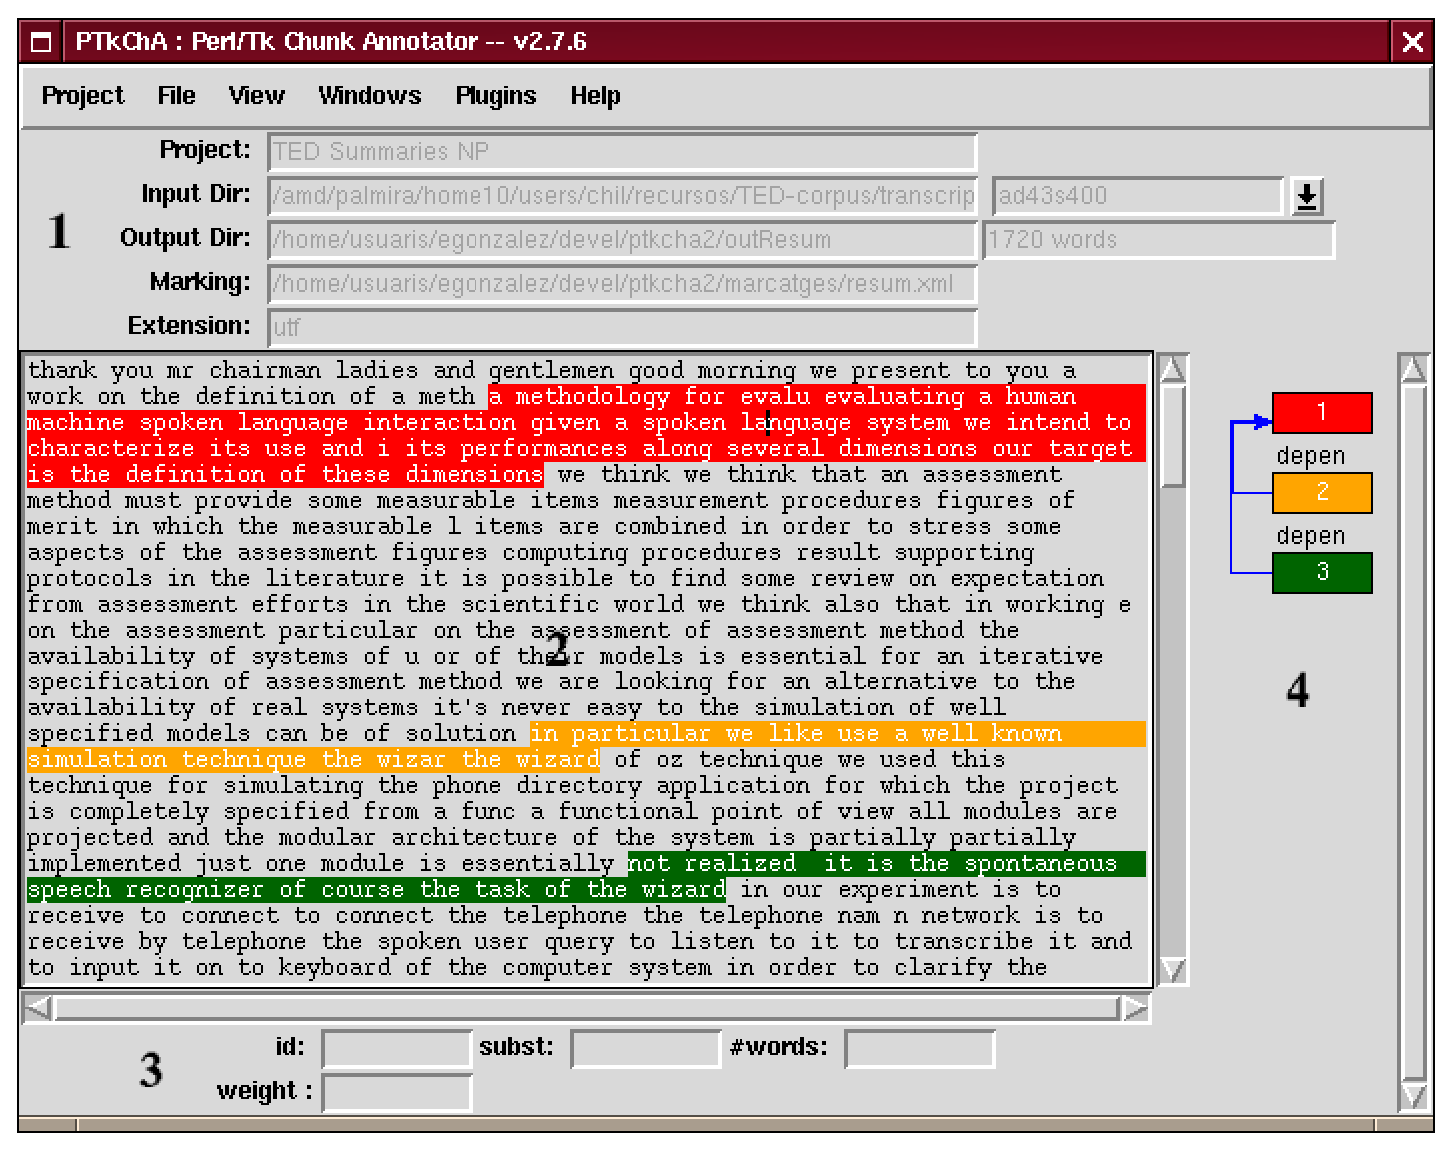
\includegraphics[width=140mm]{img/screen-annot.eps}

\caption{Main window}
\label{fig:screen}
\end{center}
\end{figure}

\begin{description}
\item[1. Project Information] Here we can see the information about
the current project, as well as select, by the combo box in the right,
one of the files to annotate it. The text under the combo shows the
number of words in the document\footnote{This number of words is just
an informative measure. It does not intend to give the precise number,
but it simply counts elements separated by whitespace}.

\item[2. Text Area] Here we can see the text of the currently selected
file, and perform several operations of it.
\begin{itemize}
\item To create new chunks, select a region of text in the usual way,
and then either press the RETURN key or click the right mouse
button. If the option \textbf{Selection Expansion} is set (see section
\ref{sec:project}) the selection is expanded so it does not include
extra whitespace beyond the first and last word of the chunk, and so
it does not finish in the middle of a word.
\item To reduce an existing chunk, select a region of text strictly
included in the chunk and do as in the previous case.
\item To expand an existing chunk, select a region of text that
overlaps but is not strictly included in the chunk, and do as in the
previous case. The chunk will grow to the union of both regions.
\item To see information about a chunk, move the pointer over it and
the information will appear on the chunk information region
(identified as 3 in figure \ref{fig:screen}).
\item To see the relations of a chunk, click the left button on it,
and the information will be shown on the relation information region
(identified as 4).
\item To edit the chunk, click the right button on it, and a pop-up
will appear, allowing us to:
  \begin{itemize}
  \item Change the values of its attributes. 
  \item Add a relation to another chunk. After selecting this option,
the cursor will change to a cross and we will be able to select the
target chunk with the left button. This can be canceled with the
ESCAPE key or by pressing the right button.
  \item Delete the chunk. This will also delete all relations having
the chunk as source or target.
  \end{itemize}
\end{itemize}

\item[3. Chunk Information] This region shows the ID and SUBST of the
chunk currently under the cursor, as well as the values of its
attributes and its length in words.

\item[4. Relation Information] This region shows the relations in
which the current chunk is involved, either as source or as
target. Clicking the left button on the boxes depicting the chunks
related, the text will scroll to locate them. Clicking the right
button, we will have access to a popup giving us the chance to delete
the relation.

\end{description}

For users with single-button mice, those operations requiring the
right button may also be performed by holding the SHIFT key while
clicking the left button.

\subsection{Menus}
\subsubsection{Project}
\label{sec:project}
\begin{description}
\item[New...] Allows the creation of a new project. The newly created
project is set as the current one.
\item[Open...] Sets a project from the list of existing ones as the
current.
\item[Delete...] Allows the deletion of an existing project. It
cannot be the current one.
\item[Options...] Allows the changing of global options:
\begin{description}
\item [Forced Writing] If a file has not been modified from its state
in the input directory, by default its counterpart in the output
directory is not written. By activating this option we can force the
output file to be written.
\item [Selection Expansion] Expands the selection when creating new
chunks, as explained in section \ref{sec:main}.
\item [Include Directories] Gives a list of additional directories to
look for the source files of plugins and filters (see sections
\ref{sec:plugins} and \ref{sec:filters}).
\end{description}
\item[Quit] Quits the program.
\end{description}

\subsubsection{File}
\begin{description}
\item[Save] Usually, changes are saved automatically whenever the
current file is changed: another one is selected, the project is
changed, the program is closed... With this command, we can force the
file to be written immediately.
\item[Revert] Allows us to lose the unsaved changes and revert to the
last saved version of the file.
\item[Initial Version] Allows us to lose all changes and come back to
the initial version of the file, that of the input directory.
\item[Default Values...] Allows the changing of the default values new
chunks will have for their attributes.
\end{description}

\subsubsection{View}
\label{sec:view}
On the Text Area, the color of every chunk may be just an identifier
of the chunk or of the cluster it belongs to (in case of a clustered
marking), or may also be a function of the value of an attribute. With
this menu we can change the current view mode. The correspondence
between colors and values can be examined using the Chart window
(section \ref{sec:windows}).

\subsubsection{Windows}
\label{sec:windows}
\begin{description}
\item[Chart] Opens a Chart window. The Chart window accomplishes a
double task: it gives the values of the attributes for every color in
the current view mode (see section \ref{sec:view}), and it also gives
the number of words in chunks with every attribute value, as well as
the fraction of the total of words in the document they represent. The
discriminant attribute in the Chart window depends on the current view
mode, selected in the \textsc{View} menu. 
\end{description}

\subsubsection{Plugins}
\label{sec:pluginmenu}
This menu is initially empty and, when a project is opened, it is
populated with the menus provided by the plugins defined in the
project's marking.

\subsubsection{Help}
\begin{description}
\item[About...] Shows a small window with information about the
program.
\end{description}

\section{Output Files}
\label{sec:output}

The output files are \emph{headless} XML files, in the sense that
there is no element that embraces the whole file. This makes them not
strictly XML-compliant, yet suitable for most practical purposes. If
XML-compliance is an issue, including the file contents in a
\texttt{<document>..</document>} pair is enough. A sample of the
contents of an output file is in figure \ref{fig:output}.

\begin{figure}[ht]

\begin{center}
\begin{minipage}{135mm}
\begin{verbatim}
thank you mr chairman ladies and gentlemen good morning we present to
you a work on the definition of a meth <summary id="1" subst="1"
weight="1">a methodology for evalu evaluating a human machine spoken
language interaction given a spoken language system we intend to
characterize its use and i its performances along several dimensions
our target is the definition of these dimensions</summary> we think we
...
looking for an alternative to the availability of real systems it's
never easy to the simulation of well specified models can be of
solution <summary id="2" subst="2" weight="1"><rels><rel type="depen"
target="1" /></rels>in particular we like use a well known simulation
technique the wizar the wizard</summary> of oz technique we used this
technique for simulating the phone directory application for this
\end{verbatim}
\end{minipage}

\caption{Sample Output File}
\label{fig:output}
\end{center}
\end{figure}

The file contains the imported text from the input directory. Each
annotated chunk is enclosed inside an XML element. The type of element
determined by the \textbf{element} attribute in the marking file (see
section \ref{sec:marking}). In the sample case, it is
\texttt{summary}. The attributes of the element are its unique ID, its
SUBST or cluster ID (only if the marking is \textbf{clustered}) and
the values for all attributes of the chunk. In the sample case, the
only attribute defined in the marking is \textbf{weight}.

If some relation has the chunk as source, immediately after the
opening tag of the chunk comes a \textbf{rels} element, which consists
of a list of \textbf{rel} elements describing the \textbf{type} and
the \textbf{target} of the relation. The target chunk is identified by
its unique ID. If there are no relations coming out of the chunk, the
\textbf{rels} element is omitted.


\section{Plugins}
\label{sec:plugins}

\ptkcha\ offers support for runtime-loading plugins, which offer
additional functionalities depending on the type of marking we are
using.

A sample of the kind of functionalities plugins may provide appears in
section \ref{sec:sumplugin}.


\section{Filters}
\label{sec:filters}

The filters allow the use of several inputs formats for the projects
in a flexible way. New filters can be added by implementing them as
Perl modules and, by now, modifying the user configuration
file. However, \ptkcha\ comes with a standard set of them.

\subsection{Standard Filters}
\begin{description}
\item [txt] The simplest filter, it performs no conversion on the
input files.
\item [yam] It reads the output of the \textsc{YamCha} \cite{kudo01}
chunker when applied to Named Entity Recognition and Classification
with the MUC classes (Person, Organization, Location and Others).
\item [utf] It reads files in Universal Transcript Format and leaves
only the spoken words information.
\item [utf\_np] It also reads Universal Transcript Format files, but in
addition, removes capitalization and punctuation information.
\end{description}

\appendix

\section{Summary Annotation Framework}
\subsection{CHIL Summary Creation Methodology}
The \cite{fuentes05a} CHIL project deliverable defined a methodology
for the creation of summaries.

From the raw text, human annotators started by identifying relevant
text fragments (chunks) and giving them a weight (1, 2 or 3) according
to their relevance. Also, chunks considered equivalent had to be
identified, as well as chunks whose presence in a summary was
dependant on the presence of another one to allow understanding.

Lastly, summaries of different sizes had to be built by selecting a
number of chunks from the relevant set.

\ptkcha\ includes a marking and a plugin for summary chunk annotation
and summary creation following this methodology.


\subsection{Summary Marking}
The summary marking defines:

\begin{description}
\item [weight] An attribute which gives the relevance of the chunk,
in a range of three values (1, 2, 3).

\item [depen] An unidirectional relation of dependency between a chunk
and another chunk which should be present in the summary if the former
is.

\item [clustered] The chunks are clustered. Those chunks belonging to
the same cluster are equivalent. Hence, only one of the chunks in a
cluster needs to be present in the summary.
\end{description}


\subsection{Summary Plugin}
\label{sec:sumplugin}
The plugin offers two main functionalities: that of generating
summaries from the annotated text and that of checking the dependency
relations. Both can be accessed through the \textsc{Plugins} menu.

\subsubsection{Generate Summary}
The interface of this plugin functionality is that of figure
\ref{fig:sumpluginscreen}.

\begin{figure}[pt]
\begin{center}
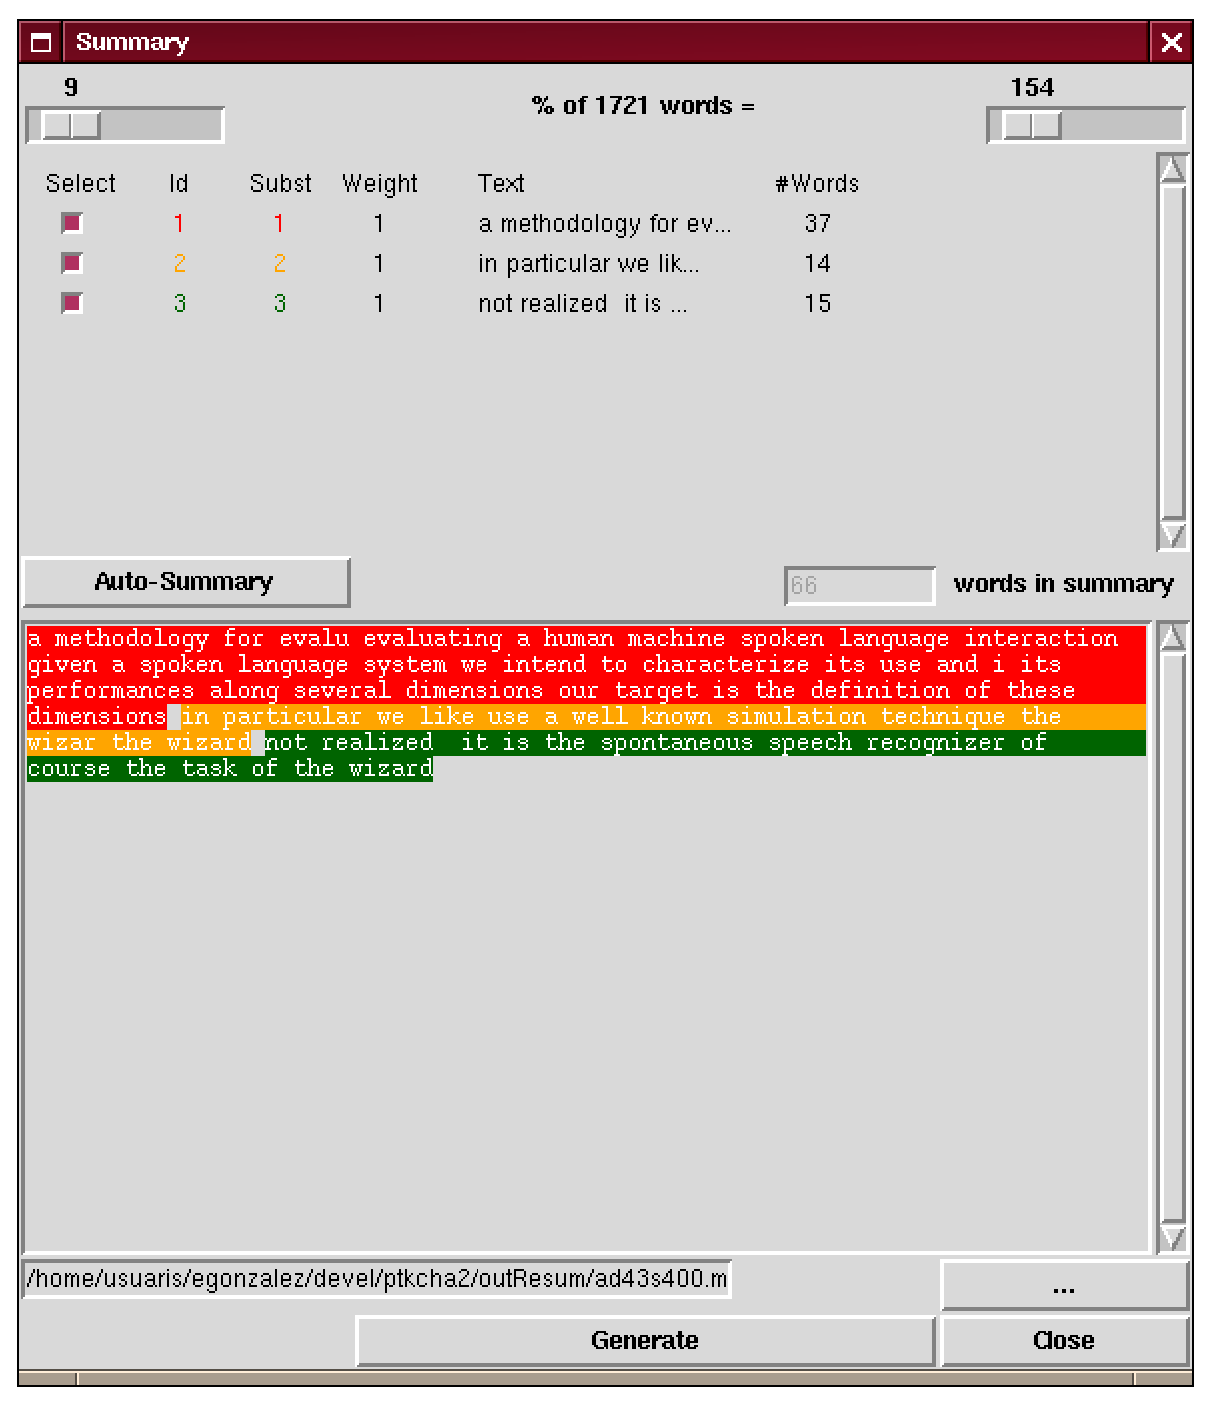
\includegraphics[width=145mm]{img/sumplugin.eps}

\caption{The Generate Summary interface}
\label{fig:sumpluginscreen}
\end{center}
\end{figure}

The slide bars on the top of the window allow to restrict the size of
the summary to a percentage of the words in the document, or to a
fixed number of words. In the middle a table with every annotated
chunk and information about it is shown. We can also select and
unselect a particular chunk to appear in the summary using the
check boxes to the left of them. The produced summary is written in the
lower part of the window, and its length is in the text entry between
the chunk table and the summary.

To the left of it, we have the \texttt{Auto-Summary} button. This
button allows us to get an automatic base summary from which to start
the selection process. This summary is built as follows:

\begin{enumerate}
\item All chunks of weight 1 are selected.
\item If we do not reach the desired number of words, all chunks of
weight 2 are also selected.
\item If we do not reach the desired number of words, all chunks of
weight 3 are also selected.
\item At every step, if a series of chunks are considered to be
equivalent, only the first one of them is selected.
\end{enumerate}

After the desired chunks are selected, we may choose a name for the
output file and generate it using the \texttt{Generate} button. Before
the generation, the set of chunks is verified, so no two equivalent
chunks be included, nor a dependency relation be broken.

We may dismiss the window using the \texttt{Close} button.

\subsubsection{Check Dependencies}
This option just checks the sanity of the \texttt{depen} relations: no
chunk should depend of another one of lower relevance. 

\subsection{Alignment Plugin}

\bibliographystyle{alpha}
\bibliography{bibliografia}

\end{document}


